\chapter{ Automatic analysis of text}
\label{chap:text}

In earlier chapters, you learned about both supervised and unsupervised machine learning as well about dealing with texts.
This chapter brings together these elements and discusses how to combine them to automatically analyze large corpora of texts. We begin with a very simple top-down approach in Section~\ref{sec:dictionary}, in which we count occurrences of words from an \emph{a priori} defined list of words. In Section~\ref{sec:supervised}, we still use pre-defined categories that we want to code, but let the machine ``learn'' the rules of the coding itself. Finally, in Section~\ref{sec:unsupervised}, we employ a bottom-up approach in which we do not use any \emph{a priori} defined lists or coding schemes, but inductively extract topics from our data.


\section{Dictionary approaches to text analysis}
\label{sec:dictionary}

A straightforward way to automatically analyze text is to compile a
list of terms you are interested in and simply count how often they
occur in each document. For example, if you are interested to find out
whether mentions of political parties in news articles change over
the years, you only need to compile a list of all party names and
write a small script to count them.

Historically, this is how sentiment analysis was
done. \refex{sentsimple} shows how to do a simple sentiment analysis
based on a list of positive and negative words. The logic is
straightforward: you count how often each positive word occurs in a
text, you do the same for the negative words, and then determine which
occur more often.


\pyrex[input=both, output=none, caption={Different approaches to a simple dictionary-based sentiment analysis: counting and summing all words using a for-loop over all reviews (Python) versus constructing a term-document matrix and looking up the words in there (R). Note that both approaches would be possible in either language.}]{chapter12/sentsimple}

As you may already realize, there are a lot of downsides to this
approach. Most notably, our bag-of-words approach does not allow us to
account for negation: ``not good'' will be counted as
positive. Relatedly, we cannot handle modifiers such as ``very
good''. Also, all words are either positive or negative, while
``great'' should be more positive than ``good''. More advanced
dictionary-based sentiment analysis packages like Vader \citep{Hutto2014},
or SentiStrength \citep{Thelwall2012} include such functionality. Yet, as we will
discuss in Section~\ref{sec:supervised}, also these off-the-shelf
packages perform very poorly in many sentiment analysis tasks,
especially outside of the domains they were developed for.
Dictionary-based sentiment analysis has been shown to be problematic
when analyzing news content \citep[e.g.][]{Gonzalez-Bailon2015,
  Boukes2019}. They are problematic when accuracy on the sentence
level is imporant, but may be satisfactory with longer texts for
comparatively easy tasks such as movie review classification
\citep{Reagan2017}, where there is clear ground truth data and the
genre convention implies that the whole text is evaluative and
evaluates one object (the film).


Still, there are many use cases where dictionary approaches work very
well. Because your list of words can contain anything, not just
positive or negative words. Dictionary approaches have been used, for
instance, to measure the use of racist words or swearwords in online
fora \citep[e.g.,][[]{Tulkens2016}. Dictionary approaches are simple to understand and
straightforward, which can be a good argument for using them when it
is important that the method is no black-box but fully transparent
even without technical knowledge. Especially when the dictionary is already
existing or easy to create, it is also a very cheap method.
However, this goes at the expense of their limitation to only performing well when measuring easy to operationalize concepts. To put it bluntly: it's great for measuring the visibility of parties or organizations in the news, but it's not
good for measuring concepts such as emotions or frames.

What gave dictionary approaches a bit of a bad name is that many
researchers applied them without validating them. This is especially
problematic when a dictionary is applied in a slightly different
domain than for which it was originally made.

If you want to use a dictionary-based approach, we advise the
following procedure:

\begin{enumerate}
  \item Construct a dictionary based on theoretical considerations and by closely reading a sample of example texts.
  \item Code some articles manually and compare with the automated coding.
  \item Improve your dictionary and check again.
  \item Manually code a validation dataset of sufficient size. The required size depends a bit on how balanced your data is -- if one code occurs very infrequently, you will need more data.
  \item Calculate the agreement. You could use standard intercoder reliability measures used in manual content analysis, but we would also advise you to calculate precision and recall (see Secion~\ref{sec:validation}).
  \end{enumerate}

Very extensive dictionaries will have a high recall (it becomes
increasingly unlikely that you ``miss'' a relevant document), but
often suffer from low precision (more documents will contain one of
the words even though they are irrelevant). Vice versa, a very short
dictionary will often be very precise, but miss a lot of documents.
It depends on your research question where the right balance lies, but
to substantially interpret your results, you need to be able to
quantify the performance of your dictionary-based approach.


\section{Supervised text analysis: automatic classification and sentiment analysis}
\label{sec:supervised}

For many applications, there are good reasons to use the dictionary
approach presented in the previous section. First, it is intuitively
understandable also for lay people, and results can -- in principle --
even be varified by hand, which can be an advantage when transparency
or communicatibility is of high importance. Second, it is very easy to
use.

Dictionary approaches excel under three conditions: First, the
variable we want to code is \emph{manifest and concrete} rather than
\emph{latent and abstract}: names of actors, specific physical
objects, specific phrases, etc., rather than feelings, frames, or
topics. Second, all synonyms to be included must be known
beforehand. And third, the dictionary entries must not have multiple
meanings.

For instance, coding how often gun control is mentioned in political
speeches fits these criteria. There are only so many ways to talk
about it, and it is rather unlikely that speeches about other topics
contain a phrase like ``gun control''. Similarily, if we want to find
references to Angela Merkel, Donald Trump, or any other well-known
politician, we can just directly search for their names -- even though
problems arise when people have very common surnames and are referred
to by their surnames only.

Sadly, most interesting concepts are more complex to code. Take a
seemingly straightforward problem: distinguishing whether a news
article is about the economy or not. This is really easy to do for
humans: there may be some edge cases, but in general, people rarely
need longer than a second to grasp whether an article is about the
economy rather than about sports, culture, etc. Yet, many of these
article won't directy state that they are about the economy by
explicitly using the word ``economy''.

We may think of extending our dictionary not only with |economi.*| (a
regular expression that includes economists, economic, and so on), but
also come up with other words like ``stock exchange'', ``market'',
``company'' -- but wait. Here, we run into a problem that we also
faced when we dicussed the precision-recall tradeoff in
Section~\ref{sec:validation}: The more terms we add to our
dictionary, the more false positives we will get: articles about
geographical space called ``market'', about some celebrity being seen
in ``company'' of someone else, and so on.

From this example, we can conclude that often (1) it is easy for
humans to decide to which class a text belongs, but (2) it is very
hard for humans to come op with a list of words (or rules) on which
their judgement is based.

Such a situation is the perfect use case for supervised machine
learing: After all, it won't take us much time to annotate, say, 1000
articles based on whether they are about the economy or not (probably
this takes less time than thoroughly finetuning a list of words to in-
or exclude); and the difficult part, deciding on the exact rules
underlying the decision to classify an article as economic is done by
the computer in seconds.


\subsection{Putting together a workflow}
With the knowledge we gained in previous chapters, it is not difficult
to set up a supervised machine learning classifier to automatically
determine, for instance, the topic of a news article.

Let us recap the building blocks that we need. In
Chapter~\ref{chap:introsml}, you learned how to use different
classifiers, how to evaluate them, and how to choose the best
settings. However, in these examples, we used numerical data as
features; now, we have text.  In Chapter [INSERT REF TO CHAPTER
  10/PROCESSING TEXT], you learned how to turn text into numerical
features. And that's all we need to get started!

Typical examples for supervised machine learning in the analysis of
communication include the classification of topics
\citep[e.g.,][]{Scharkow2011}, frames \citep[e.g.,][]{Burscher2014},
user characteristics such as gender or ideology \todo{add references},
or sentiment.

Let us consider the case of sentiment analysis more in
detail. Classical sentiment analysis is done with a dictionary
approach: you take a list of positive words, a list of negative words,
and count what occurs more. Addtionally, one may attach a weight to
each word, such that ``perfect'' gets a higher weight than ``good'',
for instance.  An obvious drawbacks include that these pure
bag-of-words approaches cannot cope with negation (``not good'') and
intensifiers ``very good''), which is why extensions have been
developed that take these (and other features, such as punctuation)
into accout \citep{Thelwall2012,Hutto2014,DeSmedt2012}.
% come back to this in crowddcoding-chapter: \citep{Haselmayer2016}

But while available off-the-shelf packages that implement these
extended dictionary-based methods are very easy to use (in fact, they
spit out a sentiment score with one single line of code), it is
questionable how well they work in practice. After all, ``sentiment''
is not exactly a clear, manifest concept for which we can enumerate a
list of words. It has been shown that results obtained with multiple
of these packages correlate very poorly with each other and with human
annotations \todo{add reference paper wouter}.

Consequently, it has been suggested that it is better to use
supervised machine learning to automatically code the sentiment of
texts \citep{Gonzalez-Bailon2015,vermeer2019seeing}. In particular,
one may need to annotate a custom, own dataset: training a classifier
on, for instance, movie reviews and then using it to predict sentiment
in political texts violates the assumption that training set, test
set, and the unlabeled data that are to be classified are (at least in
principle and approximately) drawn from the same population.

To illustrate the workflow, we will use the ACL IMDB dataset, a large
dataset that consists out of a training dataset of 25,000 movie
reviews (out of which 12,500 positives ones and 12,500 negative ones)
and an equally sized test dataset \citep{aclimdb}. It can be
downloaded at
\url{https://ai.stanford.edu/~amaas/data/sentiment/aclImdb_v1.tar.gz}


These data do not come in one file, but rather in a set of textfiles
that are sorted in different folders named after the dataset they
belong to (|test| or |train|) and their label (|pos| and |neg|). This
means that we cannot simply use a pre-defined function to read them,
but we need to think of a way of reading the content into a
datastructure that we can use. One way of doing so is shown in
\refex{readimdb}.

\pyrex[output=none, caption={Reading the ACL IMDB dataset.}]{chapter12/readimdb}


\begin{feature}
  \textbf{Sparse versus dense matrices and why it matters a lot for
    choosing between R and Python for machine learning.} In a
  document-term matrix, you would typically find a lot of zeros: most
  words do \emph{not} appear in any given document. For instance, the
  reviews in the IMDB dataset contain more than 100,000 unique
  words. Hence, the matrix has more than 100,000 columns. Yet, most
  reviews only consist of a couple of hundreds of words. As a
  consequence, more than 99\% of the cells in the table contain a
  zero. In a sparse matrix, we do not store all these zeros, but only
  store the values for cells that actually contain a value. This
  drastically reduces the memory needed.  But even if you have a huge
  amount of memory, this does not solve the issue: In R, the number of
  cells in a matrix is limited to 2,147,483,647. It is therefore
  impossible to store a matrix with 100,000 features and 25,000
  documents as a dense matrix. Unfortunately, many models that you can
  run via \pkg{caret} in R will convert your sparse document-term
  matrix to a dense matrix, and hence are effectively only usable for
  very small datasets. An alternative is using the \pkg{quanteda} package,
  which does use sparse matrices throughout. However, at the time of
  writing this book, quanteda only provides a very limited number of
  models. As all of these problems do not arise in \pkg{scikit-learn},
  you may want to consider using Python for many text classification tasks.
\end{feature}


Let us now train our first classifier. We choose a Na\"ive Bayes
classifier with a simple count vectorizer (\refex{imdbbaseline}).  In
the Python example, pay attention to the fitting of the vectorizer: we
fit on the training data \emph{and} transorm the training data with
it, but we only transform the test data \emph{without re-fitting the
  vectorizer}. Fitting, here, includes the decision which words to
include (by definition, words that are not present in the training
data are not included; but we could also choose additional
constraints, such as exluding very rare or very common words), but
also assigning an (internally used) identifier (variable name) to each
word. If we would fit the classifier again, these would not be
compatible any more. In R, the same is achieved in a slightly
different way: Two term-document matrices are created independently,
before they are matched in such a way that only the features that are
presen t in the training matrix are retained in the test matrix.


\note{A word that is not present in the training data, but is present
  in the test data, is thus ignored. If you want to use the
  information such out-of-vocabulary words can entail (e.g., they may
  be synonyms), you need to use a word embedding approach}

We do not necessarily expect this first model to be the best
classifier we could come up with, but it provides us with a reasonable
baseline. In fact, even without any further adjustments, it works
reasonably well: precision is higher for positive reviews and recall
is higher for negative reviews (classifying a positive review as
negative happens twice as much as the reverse), but none of the values
is concerningly low.

\pyrex[output=py, caption=Training a Na\"ive Bayes classifier with simple word counts as features]{chapter12/imdbbaseline}



\subsection{Finding the best classifier}

\todo[inline]{\url{https://github.com/quanteda/quanteda.textmodels} seems to be under heavy development right now. In the CRAN version of quanteda, there is only a NB classifier present. Let's wait for a moment to check which textmodels will be available via quanteda and then incorporate them here.}

Let us start by comparing two simple classifiers we know (Na\"ive
Bayes and Logistic Regression, see Section~\ref{sec:nb2dnn} and two
vectorizers that transform our texts into two numerical
representations that we know: word counts and $tf\cdot idf$ scores
[ADD REF TO CHAPTER 11].

We can also tune some things in the vectorizer, such as filtering out
stopwords, or specifying a minimum number (or proportion) of documents
in which a word needs to occur in order to be included, or the maximum
number (or proportion) of documents in which it is allowed to
occur. For instance, it could make sense to say that a word that
occurs in less than $n=5$ documents is probably a spelling mistake or
so unusual that it just unnecessarily bloats our feature matrix; and
on the other hand, a word that is so common that it occurs in moret
than 50\% of all documents is so common that it does not help us to
distinguish between different classes.

We can try all of these things out by hand by just re-running the code
from \refex{imdbbaseline} and only changing the line in which the
vectorizer is specified and the line in which the classifier is
specified. There's nothing wrong with that, but it's a bit cumbersome
and not too elegant if we want to do this for more than two or three
sections. Especially in the Python world, copy-pasting essentially the
same code is considered bad style, as it makes your code unnecessary
long and increases the likelihood of errors creeping in when you, for
instance, need to apply the same changes to multiple copies of the
code.  A more elegant approach is outlined in
\refex{basiccomparisons}: We define a function that gives us a short
summary of only the output we are interested in, and then use a
for-loop to iterate over all configurations we want to evaluate, fits
them and calls the function we defined before. In fact, with 23 lines
of code, we manage to compare four different models, while we already
needed 15 lines (in \refex{imdbbaselne}) to evaluate only one model.


\codex{chapter12/basiccomparisons.py}
\codex{chapter12/basiccomparisons.py.out}

The output of this little example gives us already quite a bit of
insight of how to tackle our specific classification tasks: First, we
see that a $tf\cdot idf$ classifier seems to be slightly but
consistently superior to a count classifier (this is often, but not
always the case). Second, we see that the logistic regression performs
better than the Na\"ive Bayes classifier (also this is often, but not
always, the case). In particular, in our case, the logistic regression
improved on the exessive misclassifcation of positive reviews as
negative, and achieves a very balanced performance.

There may be instances where one nevertheless may want to use a Count
Vectorizer with a Na\"ive Bayes classifier instead (especially if it
is too computationally expensive to estimate the other model), but for
now, we may settle on the best performing combination, logistic
regression with a $tf\cdot idf$ vectorizer. You could also try fitting
a Support Vector Machine instead, but we have little reason to believe
that our data isn't linearly separable, which means that there is
little reason to believe that the SVM will perform better. Given the
good performance we already achieved, we decide to stick to the
logistic regression for now.


We can now go as far as we like, include more models, use
crossvalidation and gridsearch (see
Section~\ref{sec:crossvalidation}), etc. However, our workflow now
consists of \emph{two} steps: fitting/transforming our input data
using a vectorizer, and fitting a classifier. To make things easier,
in scikit-learn, both steps can be combined into a so-called
pipe. \refex{chapter12/basicpipe} shows how the loop in
\refex{chapter12/basiccomparisons} can be re-written using pipes (the
result stays the same).

\codex{chapter12/basicpipe.py}

Such a pipeline lends itself very well for performing a
gridsearch. \refex{gridsearchlogreg} gives you an example.  With
|LogisticRegression?| and |TfIdfVectorizer?|, we can get a list of all
possible hyperparameters that we may want to tune. For instance, these
could be the minimum and maximum frequency for words to be included or
whether we want to use only unigrams (single words) or also bigrams
(combinations of two words, see section [ADD REFERENCE TO APPROPRIATE
  SECTIONS]). For the Logistic Regression, it may be the
regularization hyperparameter C, which applies a penalty for too
complex models.  We can simply put all values for these parameters
that we want to consider in a dictionary, with as key a string with
the step of the pipeline followed by two underscores and the name of
the hyperparameter, and a list of all values we want to consider as
corresponding value.

The gridsearch procedure will then estimate all combinations of all
values, using cross-validation (see Section~\ref{sec:validation}). In
our example, we have $2 \cdot 2 \cdot 2 \cdot 2 \cdot 3 = 24$
different models, and $24$ models $\cdot 5$ folds $= 120$ models to
estimate. Hence, it can take you some time to run the code
\codex{chapter12/gridsearchlogreg.py}
\codex{chapter12/gridsearchlogreg.py.out}

We see that we could further improve our model to precision and recall
values of .90, by excluding extremely infrequent and extremely
frequent words), including both unigrams and bigrams (which, we may
speculate, helps us accounting for the ``not good'' vs ``not'',
``good'' problem), and changing the default penalty of C=1 to C=100.

Let us, just for the sake of it, compare the performance of our model
with an off-the-shelf sentiment analysis package, in this case Vader
\citep{Hutto2014}. For any text, it will directly estimate sentiment
scores (more specifically, a positivity score, a negativity score, a
neutrality score, and a compound measure that combines them), without
any need to have training data. However, as \refex{vader} shows, such
a method is clearly inferior to a supervised machine learning
approach. While in almost all cases (except $n=11$), Vader was able to
make a choice (getting scores of 0 is a notorious problem in very
short texts), precision and recall are clearly worse than even the
simple baseline model we started with, and much worse than those of
the final model we finished with. In fact, we miss half (!) of the
negative reviews. There are probably very few applications in the
analysis of communication in which we would find this acceptable.
It is important to highlight that this is not because the off-the-shelf
package we chose is a particularly bad one (on the contrary, it is
actually comparatively good), but because of the inherent limitations
of dictionary-based sentiment analysis.

\codex{chapter12/vader.py}
\codex{chapter12/vader.py.out}

We need to keep in mind, though, that with this dataset, we chose one
of the easiest sentiment analysis tasks: a set of long, rather formal
texts (compared to informal short social media messages), that
evaluate exactly one entity (one film), and that are not ambigous at
all. Many applications that communications scientists are interested
in are much less straight-forward. Therefore, how tempting it may be
to use an off-the-shelf package, doing so requires a thorough test
based on at least some human-annotated data.



\subsection{Using the model}

So far, we have focused on training and evalualting models, almost
forgetting why we were doing this in the first place: to use them to
predict the label for new data that we did not annotate.

Of course, we could always re-train the model when we need to use it
-- but that has two downsides: first, as you may have seen, it may
actually take considerable time to train it, and second, you need to
have the training data available, which may be a problem both in terms
of storage space and of copyright and/or privacy if you want to share
your classifier with others.

Therefore, it makes sense to save both our classifier and our
vectorizer to a file, so that we can reload them later
(\refex{reuse}). Keep in mind that you need not to re-use \emph{both}
-- after all, the feature matrix (e.g., which features (=words) are
included, and in which column which feature is) will be different when
fitting a new vectorizer. Therefore, as you see, you do not do any fitting any more, and only use the |.transform()| method of the (already fitted) vectorizer and the |.predict()| method of the (already fitted) classifier.

\pyrex[output=py, caption=Saving and loading a vectorizer and a classifier]{chapter12/reuse}



Another thing that we might want to do is to get a better idea of the
features that the model uses to arrive at its prediction; in our
example, what actually characterizes the best and the worst
reviews. \refex{eli5} shows how this can be done in one line of code
using eli5 -- a model that aims to ``\emph{e}xplain [the model]
\emph{l}ike \emph{I}'m \emph{5} years old''. Here, we re-use the
|pipe| we constructed earlier to provide both the vectorizer and the
classifier to the eli5 -- if we would have only provided the
classifier, than the feature names would have been internal
identifiers (which are meaningless to us) rather than human-readable
words.

\pyrex[output=py, format=html, caption=Using ELI5 to get the most predictive features]{chapter12/eli5}

We can also use eli5 to explain how the classifier arrived at a
prediction for a specific document, by using different shades of green
and red to explain how much different features contributed to the
classification, and in which direction (\refex{eli5b}).

\pyrex[output=py, format=html, caption=Using ELI5 to explain a prediction]{chapter12/eli5b}


\todo[inline]{Include an example of RNN to text classification}



\section{Unsupervised text analysis: topic modeling}
\label{sec:unsupervised}

In \refsec{clustering}, we discussed how clustering techniques can be used to find patterns in data,
such as which cases or respondents are most similar.
Similarly, especially in survey research it is common to use factor analysis to discover (or confirm) variables that form a scale.

In essence, the idea behind these techniques is similar:
by understanding the regularities in the data (which cases or variables behave similarly),
you can describe the relevant information in the data with fewer data points.
Moreover, assuming the regularities capture interesting information and the deviations from these regularities are mostly
uninteresting noise, these clusters of cases or variables can actually be substantively informative.

Since a document-term matrix (DTM) is `just' a matrix, you can also apply these clustering techniques to the DTM
to find groups of words or documents. You can therefore use any of the techniques we described in \refchap{eda}, and in particular clustering techniques such as $k$-means clustering (see  \refsec{clustering}) to group documents that use similar words together. 

It can be very instructive to do this, and we encourage you to play around with such techniques. However, in recent years, a set of models called \concept{topic models} have become especially popular for the unsupervised analysis of texts. Very much what like what you would do with other unsupervised techniques, also in topic modeling, you group words and documents into `topics', consisting of words and documents that co-vary.
If you see the word `agriculture' in a news article, there is a good chance you might find words such as `farm' or `cattle',
and there is a lower chance you will find a word like `soldier'.
In other words, the words `agriculture' and `farm' generally occur in the same kind of documents, so they can be said to be part of the same topic.
Similarly, two documents that share a lot of words are probably about the same topic,
and if you know what topic a document is on (e.g. an agricultural topic), you are better able to guess what words might occur in that document (e.g. `cattle')

Thus, we can formulate the goal of topic modeling as: given a corpus, find a set of N topics, consisting of specific words and/or documents, that minimize the mistakes we would make if we try to reconstruct the corpus from the topics.
This is similar to regression where we try to find a line that minimizes the prediction error.

In early research on document clustering, a technique called Latent Semantic Analysis (LSA) essentially used a factor analysis technique called Singular Value Decomposition (see \refsec{pcasvd} on the DTM.
This has yielded promising results in information retrieval (i.e. document search) and studying human memory and language use.
However, it has a number of drawbacks including factor loadings that can be difficult to interpret substantively and no good way of dealing with words that can have multiple meanings \citep{lsa}.

\subsection{Latent Dirichlet Allocation (LDA)}

The most widely used technique for topic modeling is Latent Dirichlet Allocation (LDA).
Although the goal of LDA is the same as for clustering techniques, it starts from the other end with what is called a \concept{generative model}.
A generative model is a (simplified) formal model of how the data is assumed to have been generated.
For example, if we would have a standard regression model predicting income based on age and education level,
the implicit generative model is that to determine someone's income, you take their age and education level,
multiply them both by their regression parameters, and then add the intercept and some random error.
Of course, we know that's not actually how most companies determine wages, but it can be a useful starting point to analyse e.g. labour market discrimination.

The generative model behind LDA works as follows.
Assume that you are a journalist writing a 500 word news item.
First, you would choose one or more \emph{topics} to write about,
for example 70\% healthcare and 30\% economy.
Next, for each word in the item, you randomly pick one of these topics based on their respective weight.
Finally, you pick a random word from the words associated with that topic,
where again each word has a certain probabibility for that topic.
For example, `hospital' might have a high probability for healthcare while `effectiveness' might have a lower probability but could still occur.

As said, we know (or at least strongly suspect) that this is not how journalists actually write their stories.
However, this generative model helps understand the substantive interpretation of topics.
Moreover, LDA is a \concept{mixture model}, meaning it allows for each document to be about multiple topics, and for each word to occur in multiple topics.
This matches with the fact that in many cases, our documents are in fact about multiple topics,
from a news article about the economic effects of the COVID virus to an open survey answer containing multiple reasons for supporting a certain candidate. 
Additionally, since topic assignment is based on what other words occur in a document,
the word `pupil' could be assigned either to a `biology' topic or to an `education' topic, depending
on whether the document talks about eyes and lenses or about teachers and classrooms.

\begin{figure}
  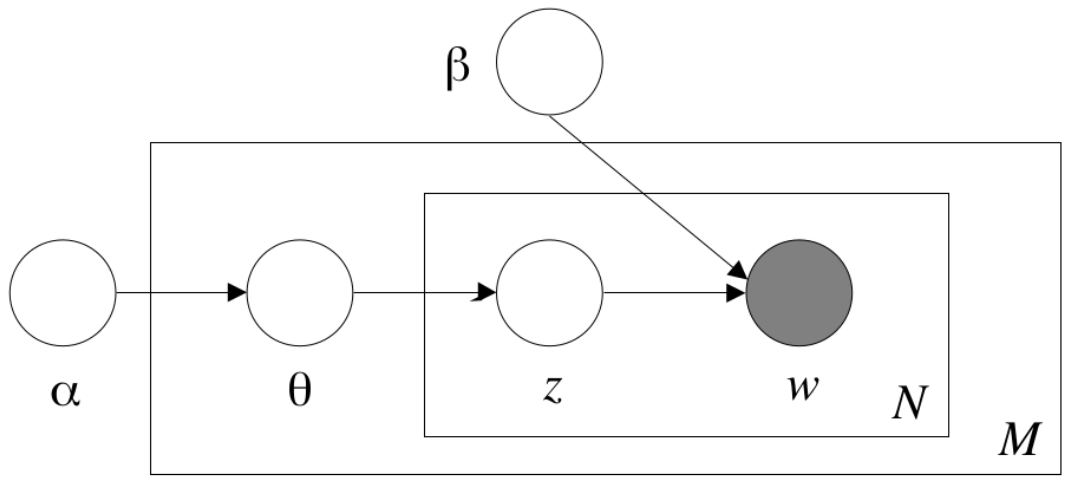
\includegraphics[width=\linewidth]{chapter12/lda.png}
  \caption{Latent Dirichlet Allocation in `Plate Model' notation \citep[fig. 1]{blei03}}\label{fig:lda}
\end{figure}

\reffig{lda} is a more formal notation of the same generative model.
Starting from the left, for each document you pick a set of topics $\Theta$.
This set of topics is drawn from a \concept{Dirichlet distribution} which itself has a parameter $\alpha$
(see note).
Next, for each word you select a single topic $z$ from the topics in that document.
Finally, you pick an actual word $w$ from the words in that topic, again controlled by a paramter $\beta$ (see note).

Now, if we would know which words and documents are in which topics, we could start generating the documents in the corpus.
In reality, of course, we have the reverse situation:
we know the documents, and we want to know the topics.
Thus, the task of LDA is to find the parameters that have the highest chance of generating these documents.
Since only the word frequencies are observed, this is a latent variable model where we want to find the
most likely values for the (latent) topic $z$ for each word in each document. 

Unfortunately, there is no simple analytic solution to calculate these topic assignments
like there is for OLS regression.
Thus, like other more complicated statistical models such as multilevel regression,
we need to use an iterative estimation that progressively optimizes the assignment to improve the fit until it converges.

An estimation method that is often used for LDA is Gibbs sampling.
Simply put, this starts with a random assignment of topics to words.
Then, each iteration, it reconsiders each words and recomputes what likely topics for that word are
given the other topics in that document and the topics that word occurs in  other documents.
Thus, if a document already contains a number of words placed in a certain topic,
a new word is more likely to be placed in that topic as well.
After enough iterations, this converges to a solution. 

\note{\textbf{The Dirichlet Distribution and its Hyperparameters}
  The Dirichlet distribution can be seen as a distribution over multinomial distributions,
  that is, every draw from a dirichlet distribution results in a multinomial distribution.
  An easy way to visualize this is to see the dirichlet distribution as a bag of dice.
  You draw a die from the bag, and each die is a distribution over the numbers one to six.

  This distribution is controlled by a parameter called alpha ($\alpha$),
  which is often called a \concept{hyperparameter} because it is a parameter that controls how other parameters
  (the actual topic distributions) are estimated, similar to e.g. the learning speed in many machine learning models.
  This alpha hyperparameter controls what kind of dice there are in the bag.
  A high alpha means that the dice are generally fair, i.e., give a uniform multinomial distribution.
  For topic models, this means that documents will in general contain an even spread of multiple topics.
  A low alpha means that each die is unfair in the sense of having a strong preference for some number(s), as if these numbers are weighed down. You can then draw a die that prefers ones, or a die that prefers sixes.
  For topic models this means that each document tends to have one or two dominant topics.
  Finally, alpha can be symmetric (meaning dice are unfair, but randomly, so in the end each topic has the same chance)
  or asymetric (they are still unfair, and now also favour some topics more than others).
  This would correspond to some topics being more likely to occur in all documents.
  
  In our experience, most documents actually do have one or two dominant topics,
  and some topics are actually more prevalent across many documents then others
  -- especially if you consider that procedural words and boilerplate also need to be fit into a topic unless they are filtered out beforehand.
  Thus, we would generally recommend a relatively low and asymmetric alpha,
  and in fact Gensim provides algorithm to find, based on the data, an alpha that corresponds to this recommendation (by specifying \texttt{alpha='auto'}).
  In R, we would recommend picking a lower alpha than the default value, probably around $\alpha=5/K$,
  and optionally try using an asymmetric alpha if you find some words that occur across multiple topics. 

  To get a more intuitive understanding of the effects of alpha,
  please see \url{http://cssbook.net/lda} for additional material and visualizations.
  }

\subsection{Fitting an LDA model}


\begin{ccsexample}
\doublecodex{chapter12/lda1}
\codex[caption=Output (from R)]{chapter12/lda1.r.out}
\doublecodex{chapter12/lda2}
\codexoutputtable{chapter12/lda2.r}
\caption{LDA Topic Model of Obama's State of the Union speeches}\label{ex:lda}
\end{ccsexample}

\refex{lda} shows how you can fit an LDA model in Python or R.
As example data, we use Obama's State of the Union Speeches using the corpus introduced in \refchap{dtm}.
Since such a speech generally touches on many different topics, we choose to first split by paragraph
as these will be more semantically coherent (for Obama, at least).
In R, we use the \fn{corpus\_reshape} function to split the paragraphs,
while in Python we use \pandas' \fn{str.split}, which creates a list or paragraphs for each text,
which we then convert into a paragraph per row using \fn{explode}.
Converting this to a DTM we get a reasonably sized matrix of 738 paragraphs and 746 unique words.

Next, we fit the actual LDA model using the package \pkg{gensim} (Python) and \pkg{topicmodels}.
Before we can do this, we need to convert the DTM format into a format accepted by that package.
For Python, this is done using the \fn{Sparse2Corpus} helper function while in R this is done with the \quanteda\ \fn{convert} function.
Then, we fit the model, asking for 10 topics to be identified in these paragraphs.
There are three things to note in this line.
First, we specify a \concept{random seed} of 123 to make sure the analysis is replicable.
Second, we specify an `asymmetric' of \verb|1/1:10|, meaning the first topic has alpha 1, the second 0.5, etc (in R).
In Python, instead  of using the default of \verb|alpha='symmetric'|, we set  \verb|alpha='asymmetric'|, which uses the formula
$\frac{1}{topic\_index + \sqrt{num\_topics}}$ to determine the priors. At the cost of a longer estimation time, we can even
specify \verb|alpha='auto'|, which will learn an asymetric prior from the data. For more background, see the note on hyperparameters for more information. 
Third, for Python we also need to specify the vocabulary names since these are not included in the DTM.

The final line generates a data frame of top words per topic for first inspection
(which in Python requires separating the words from their weights in a list comprehension and converting it to a dataframe for easy viewing).
As you can see, most topics are interpretable and somehwat coherent: For example, topic 1 seems to be about education and jobs,
while topic two is health care. You also see that the word `job' occurs in multiple topics (presumably because unemployment was a pervasive concern during Obama's tenure).
Also, some topics like topic 3 are relatively more difficult to interpret from this table.
A possible reason for this is that not every paragraph actually has policy content.
For example, the first paragraph of his first State of the Union was:
\emph{`Madam Speaker, Mr. Vice President, Members of Congress, the First Lady of the United States -- she's around here somewhere'}.
None of these words really fit a `topic' in the normal meaning of that term,
but all of these words need to be assigned a topic in LDA.
Thus, you often see `procedural' or `boilerplate' topics such as topic 3 occurring in LDA outputs. 

Finally, note that we showed the R results here. As \pkg{gensim} uses a different estimation algorithm
(and \sklearn\ uses a different tokenizer and stopword list), results will not be identical,
but should be mostly similar. 

\subsection{Analysing topic model results}

\begin{ccsexample}
\doublecodex{chapter12/ldaresults1}
\codexoutputtable{chapter12/ldaresults1.r}
\doublecodex{chapter12/ldaresults2}
\codex[caption=Output (from R)]{chapter12/ldaresults2.r.out}
\caption{Analysing and inspecting LDA results}\label{ex:ldaresults}
\end{ccsexample}


\refex{ldaresults} shows how you can combine the LDA results (topics per document)
with the original document metadata.
This could be your starting point for substantive analyses of the results,
for example to investigate relations between topics or between e.g. time or partisanship and topic use.

You can also use this to find specific documents for reading.
For example, we noted above that topic 3 is difficult to interpret.
As you can see in the table in \refex{ldaresults} (which is sorted by value of topic 3),
most of the high scoring documents are the first paragraph in each speech,
which do indeed contain the ``Madam speaker'' boilerplate noted above.
The other three documents are all calls for bipartisanship and support.
As you can see from this example, carefully inspecting the top documents for each topic
is very helpful for making sense of the results.


\subsection{Validating and inspecting topic models}

As we saw in the previous subsection, running a topic model is relatively easy.
However, that doesn't mean that the resulting topic model will always be useful.
As with all text analysis techniques, \concept{validation} is the key to good analysis:
are you measuring what you want to measure? And how do you know?

For topic modeling (and arguably for all text analysis),
the first step after fitting a model is inspecting the results and establishing face validity.
Top words per topic such as listed above are a good place to start with this,
but we would really encourage you to also look at the top documents per topic to better understand how words are used in context.
Also, it is good to inspect the relations between topics and look at documents that load high on multiple topics to understand the relation.

If the only goal is to get an explorative understanding of the corpus,
for example as a first step before doing a dictionary analysis or manual coding,
just face validity is probably sufficient.
For a more formal validation, however, it depends on the reason for using topic modeling.

If you are using topic modeling in a true unsupervised sense, i.e. without a predefined analytic schema in mind,
it is difficult to assess whether the model measures what you want to measure --
because the whole point is that you don't know what you want to measure.
That said, however, you can have the general criteria that the model needs to achieve \emph{coherence}
and \emph{interpretability}, meaning that words and documents that share a topic
are also similar semantically. 

In their excellent paper on the topic, \citet{chang09} propose two formal tasks to judge this
using manual (or crowd) coding: in \emph{word intrusion}, a coder is asked to pick the `odd one out' from a list
where one other word is mixed in a group of topic words.
In \emph{topic intrusion}, the coder is presented with a document and a set of topics that occur in the document,
and is asked to spot the one topic that was not present according to the model.
In both tasks, if the coder is unable to identify the intruding word or topic, apparently the model does not fit
our intuitive notion of `aboutness' or semantic similarity.
Perhaps their most interesting finding is that goodness-of-fit measures like perplexity\footnote{Perplexity is measure to compare and evaluate topic models using log-likelihood in order to estimate how well a model predicts a sample.} 
are actually not good predictors of the interpretability of the resulting models.

If you are using topic models in a more confirmatory manner,
that is, if you wish the topics to match some sort of predefined categorization,
you should use regular gold standard techniques for validation:
code a sufficiently large random sample of documents with your predefined categories,
and test whether the LDA topics match those categories.
In general, however, in such cases it is a better idea to use a dictionary or supervised analysis technique
as topic models often do not exactly capture our categories. After all, unsupervised techniques mainly
excel in bottom-up and explorative analyses.


\subsection{Beyond LDA}

This chapter focused on regular or `vanilla' LDA topic modeling.
Since the seminal publication, however, a large amount of variations and extensions on LDA have been proposed.
These include, for example, dynamic topic models (which incorporate time; \cite*{dynamiclda}),
correlated topic models (which explicitly model correlation between topics; \cite{correlatedlda}).
Although it is beyond the scope of this book to describe these models in detail,
the interested reader is encouraged to learn more about these models.

Especially noteworthy are \concept{Structural Topic Models} (R package \pkg{stm}; \cite*{stm}),
which allow you to model covariates as topic or word predictors.
This allows you, for example, to model topic shifts over time or
different words for the same topic based on e.g. Republican or Democrat presidents. 

Python users should check out Hierarchical Topic Modeling \citep{hierarchicallda}.
In hierarchical topic modeling, rather than the researcher specifying a fixed number of topics,
the model returns a hierachy of topics from few general topics to a large number of specific topics,
allowing for a more flexible exploration and analysis of the data. 




